
\documentclass[a4paper]{article}

%%%%%%%%%%%%
% Packages %
%%%%%%%%%%%%

\usepackage[english]{babel}
\usepackage[noheader]{packages/sleek}
\usepackage{packages/sleek-title}
\usepackage{packages/sleek-theorems}
\usepackage{packages/sleek-listings}

%%%%%%%%%%%%%%
% Title-page %
%%%%%%%%%%%%%%

\logo{./resources/pdf/UdeM-logo.pdf}
\institute{Université de Montréal}
%\faculty{}
\department{Département d'informatique et de recherche opérationnelle \\ (DIRO)}
\title{Génération automatique de rapports de projets ReliS}
%\subtitle{With a sleeker title-page} 

\author{\textit{Auteur}\\Soilihi \textsc{BEN SOILIHI BOINA}}

\supervisor{Professeur\\ Eugene \textsc{Syriani}}
%\context{Well, I was bored...}
\date{Novembre 29, 2020}


%%%%%%%%%%%%%%%%
% Bibliography %
%%%%%%%%%%%%%%%%

\addbibresource{./resources/bib/references.bib}


%%%%%%%%%%
% Others %
%%%%%%%%%%

\lstdefinestyle{latex}{
    language=TeX,
    style=default,
    %%%%%
    commentstyle=\ForestGreen,
    keywordstyle=\TrueBlue,
    stringstyle=\VeronicaPurple,
    emphstyle=\TrueBlue,
    %%%%%
    emph={LaTeX, usepackage, textit, textbf, textsc}
}

\FrameTBStyle{latex}

\def\tbs{\textbackslash}

%%%%%%%%%%%%
% Document %
%%%%%%%%%%%%

\begin{document}

\maketitle

\begin{abstract}
    
    Avant d'entamer une recherche quelconque, les chercheurs sont tenus de faire des revues systématiques pour se documenter le plus possible dessus. Notamment, pour savoir ce qui a déjà été fait par rapport à celle ci par exemple et, ainsi, savoir vers quelle direction mener les recherches et leurs réflections. 
       Étant donné que la construction d'une revue systématique peut être une tâche très ardue en fonction du sujet de recherche, plusieurs outils sont mis en place pour cette fin dont ReliS. 
    Cependant, dans ce dernier, bien que structurées, toutes les données ne sont pas forcément faciles à comprendre et ne sont pas forcément tous aux mêmes endroits. Il faut donc les réunir manuellement entre les phases du screening et la classification par exemple. 
    Notre travail propose de rassembler les données d'un projet dans un seul rapport généré automatiquement qui, en plus de donner des détails de ce que signifient les données, les structurera de manière claire et facile de compréhension.
    Pour se faire, dans notre approche, on recherche les projets qu'on a effectué dans ReliS à partir de son nom d'utilisateur dans notre plate-forme web, suite à quoi on choisit un projet, ce qui générera le code correspondant qui lui même sera utilisé pour générer le rapport du projet choisi. 
\end{abstract}

\newpage

\tableofcontents

\newpage

\section{Introduction}
\vspace*{0.5cm}
\hspace*{1cm} Les revues systématiques sont incontournables lorsqu'on entame un sujet de recherche pour, notamment, savoir les travaux déjà existants pour ne pas les refaire par exemple, et aussi diriger la recherche. Faire une revue systématique n'est pas une tâche aisée. C'est pour cela que de nombreux outils existent pour automatiser le processus afin de gagner en productivité, en efficacité et produire des revues systématiques très qualitatives. \\
Parmi ces outils, se hisse \textbf{ReliS}, un outil qui permet de réaliser des revues de qualité en utilisant une approche centrée sur l'ingénierie dirigée par les modèles.
Toutefois, autant qu'il est difficile de construire une revue, autant que ça peut le devenir de comprendre une revue. Dans ReliS, les données sont structurés mais les rapports sont fait pour chaque phase du screening et aussi des statistiques de la classification mais toutes ces données ne se trouvent pas aux mêmes endroits ce qui peut rendre un peu moins claire la compréhension du tout. La contribution de notre travail est de rassembler toutes les données d'un projets, à savoir, ceux de chaque phase du screening, ceux de la classification en un seul document structuré avec quelques explications en plus pour aider à la compréhension de manière automatique. \\
Nous verrons dans cet article une généralité sur les revues systématiques, un exemple de revue dans ReliS qu'on va utiliser tout le long, notre approche, la mise en oeuvre, l'évaluation de notre solution, la constitution du rapport généré, une discussion sur l'approche puis les travaux connexes, suite à quoi nous concluerons.

\newpage

\section{Les revues systématiques}
\vspace*{4mm} 

\subsection{Les types de revues systématiques}

En fonction de ce qu'on veut faire, une revue systématique peut prendre deux formes comme le cite \cite{brice}. Elle peut notamment se présenter sous la forme: 
\begin{itemize}
\item d'une \textbf{SLR(Systematic Literature Review):} ici, elle collecte des études primaires, en fait un tri de synthèse et ensuite une analyse pour donner des conclusions.
\item ou d'une \textbf{SMS(Systematic Mapping Study):} celle ci est faite pour des fins de classifications pour montrer les tendances des recherches, les outils les plus utilisés par exemple.
\end{itemize} 
\vspace*{2mm} 

\subsection{Définition d'une revue systématique}

Pour mettre en place une revue, on peut passer par plusieurs sous-étapes qu'on pourrait résumer en trois grandes étapes:
   
\begin{description}
    \item[la collecte des articles : ] des études primaires de différentes sources concernant le sujet sont collectionnées pour les faire prendre part à la revue. On Cherche ici à entrer un maximum d'article en rapport avec le sujet. Dans Relis, les articles peuvent provenir de plusieurs sources comme \textit{ACM Digital library, Springer link...etc} et tant d'autres.
    \item[Le screening :] ici, c'est l'étape la plus importante parce qu'un screening mal fait aura un impact significatif sur tout le reste. C'est ici qu'on filtre les articles. Le screening dans ReliS peut être divisé en plusieurs phases. Étant donné qu'un projet peut regrouper plusieurs chercheurs, chacun d'eux peut inclure et exclure des articles dans chaque phase. On peut aussi y définir des critères d'exclusion pour exclure automatiquement des articles. \\
    Il arrive toutefois des cas où un chercheur, dans une phase donnée, inclut une étude qu'un autre chercheur a exclus. Ce qui peut créer des conflits. Et donc, dans la phase du screening en question, il faut résoudre ces conflits. Chaque phase a ses propres résultats regroupant les inclusions et les exclusions notamment. La totalité de ces phases va constituer le screening.
    \item[La classification :] c'est la finalité de l'étude. C'est ici qu'on va répondre aux questions initialement prévues pour l'étude. Les données de la classification sont les résultats d'une étude tandis que le screening serait plutôt la démarche vers le résultat cherché.
\end{description}

\newpage

\section{Exemple d'une revue systématique dans ReliS}

Nous allons prendre comme exemple tout au long de cet article la revue systématique définie sur ReliS intitulée \textit{\textbf{"Xtext grammar"}} \footnotemark[1]. On a choisi cette revue parce qu'elle est complète( elle a eu un screening et une classification) et peut être prise à titre d'exemple. \\ \\

L'image qui suit montre une vue d'ensemble des étapes d projet dans ReliS:
\begin{figure}[H]
        \centering
        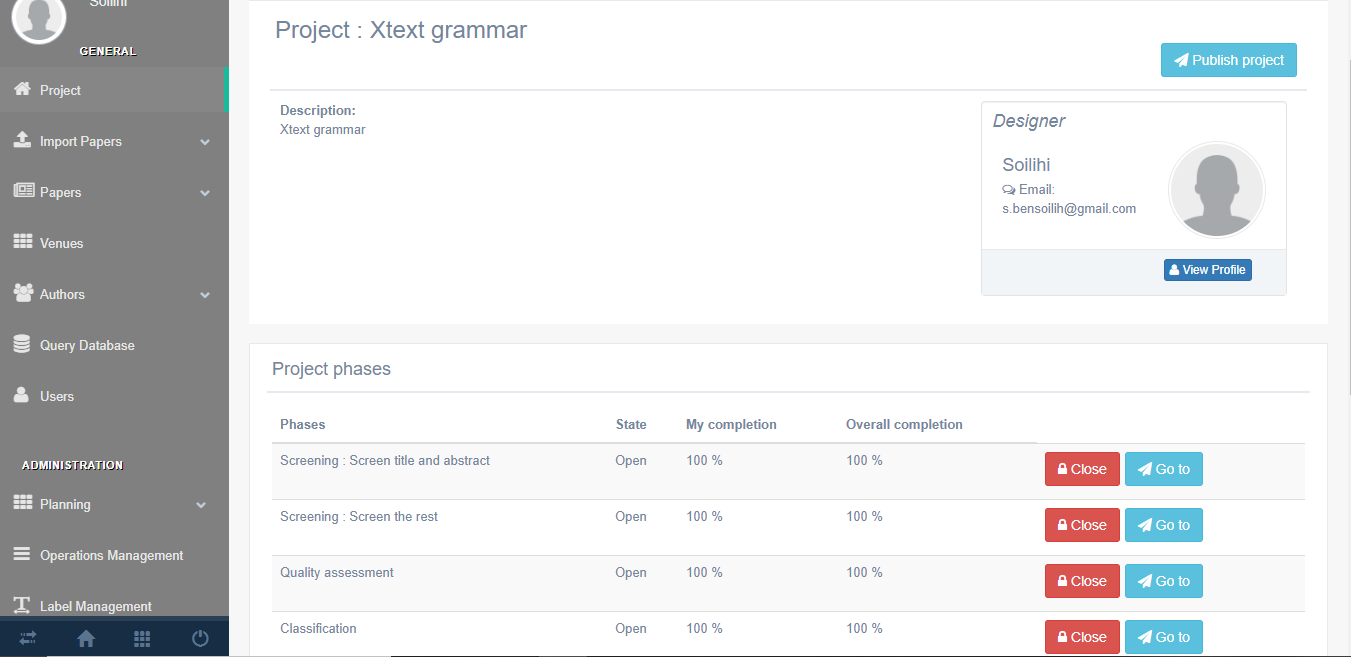
\includegraphics[width=0.65\textwidth]{resources/images/Xtext grammar.PNG}
        \noskipcaption{Project Xtext Grammar.}
    \end{figure}

Dans Relis, ce projet est constitué comme suit:

\begin{description}
    \item[La collecte :] on a inclus dans ce projet un total de 5 articles provenant de différentes sources.
    
    \item[Le screening :] on a divisé le screening en deux phases:
                        \begin{itemize}
                            \item \textcolor{blue}{{\textit{Screen title and abstract:}}} ici, on a inclus 4 articles et exclu 1 avec un critère de sélection. la figure suivante résume les données de cette phase.
     \begin{figure}[H]
        \centering
        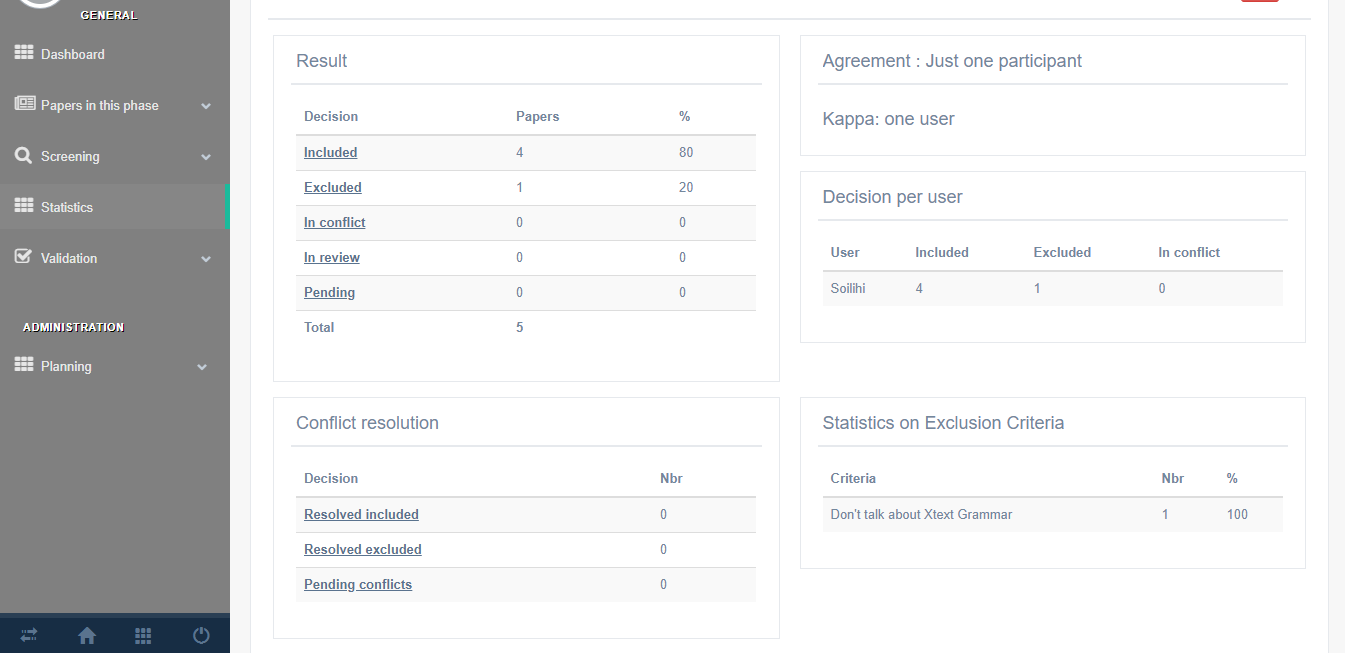
\includegraphics[width=0.65\textwidth]{resources/images/Screen title and abstract.PNG}
        \noskipcaption{Screen title and abstract.}
    \end{figure}
\newpage
                            \item \textcolor{blue}{{\textit{Screen the rest:}}} dans cette phase, on n'exclut rien et on a inclus les articles non exclus de la phase précédente. la figure suivante résume les données de cette phase.
     \begin{figure}[H]
        \centering
        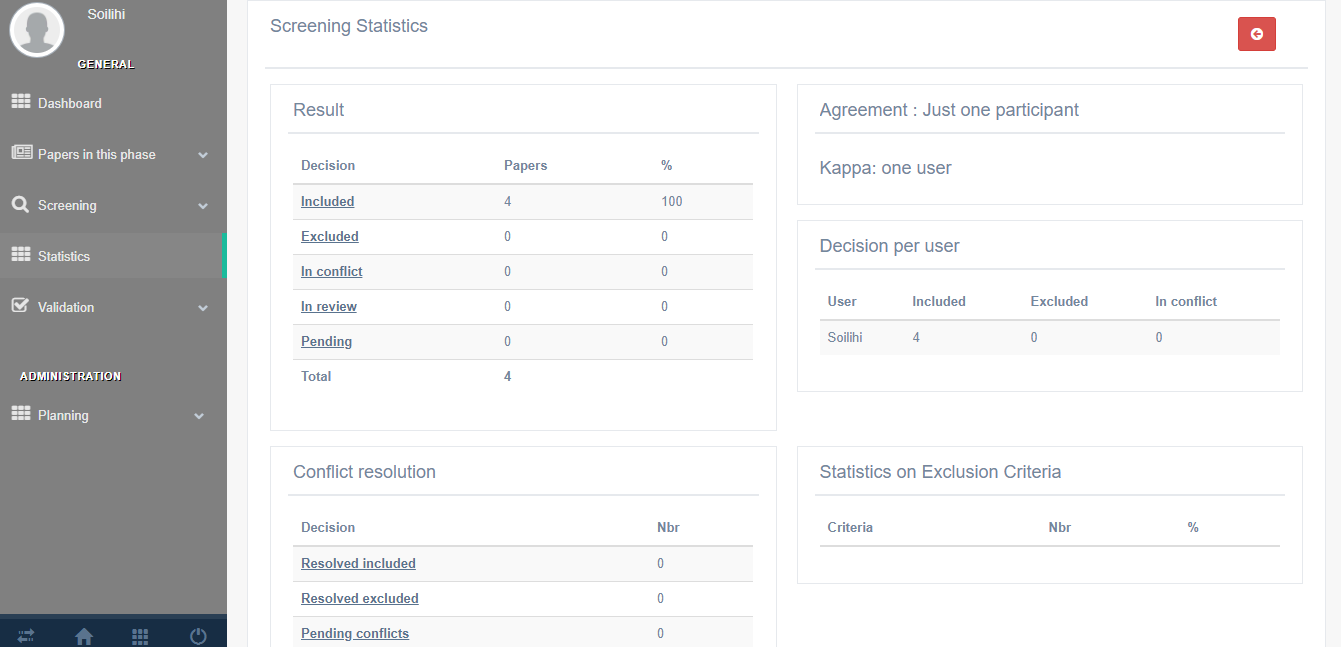
\includegraphics[width=0.65\textwidth]{resources/images/Screen the rest.PNG}
        \noskipcaption{Screen the rest.}
    \end{figure}
                        \end{itemize}            
        \item[La classification :] dans la classification, on a juste cherché à savoir si les articles restants des phases précédentes du screening parlait de Xtext, ce qui est le cas des 4 articles, soit leur totalité après le filtre du screening. L'image qui suit illustre les données de la classification.
        \begin{figure}[H]
        \centering
        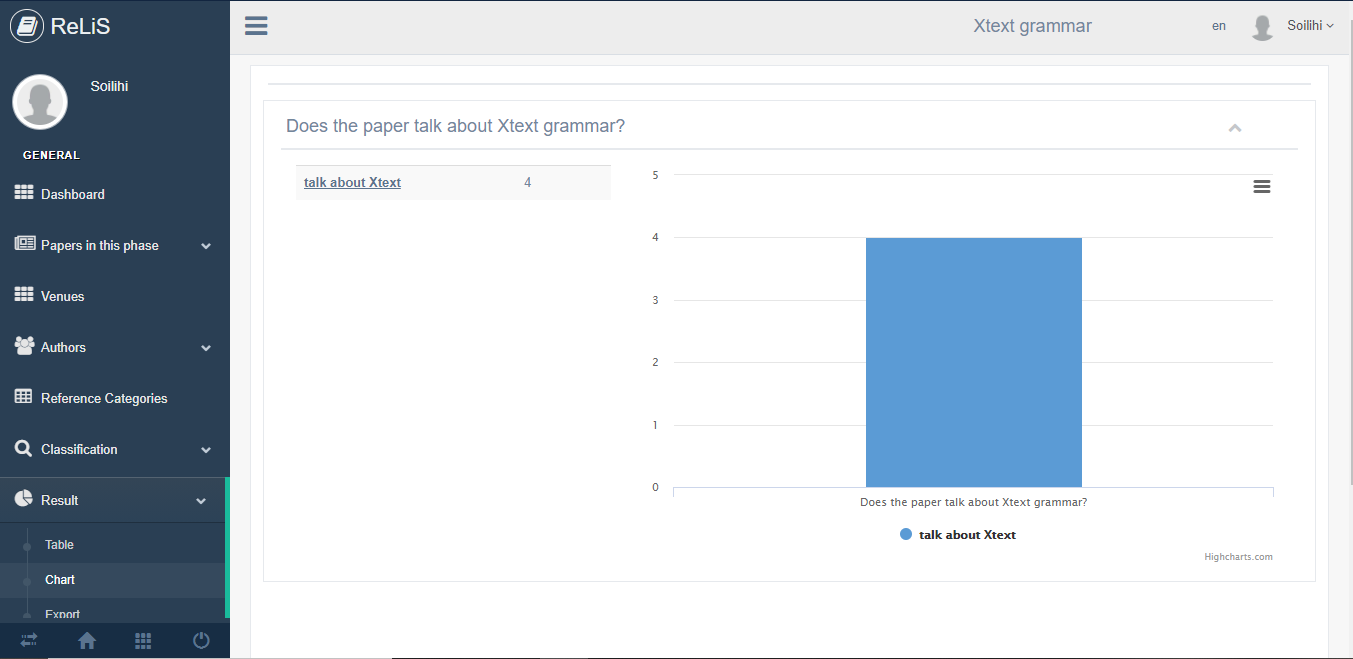
\includegraphics[width=0.65\textwidth]{resources/images/classification.PNG}
        \noskipcaption{Classification.}
    \end{figure}
\end{description}

\footnote[1]{ Ce projet \textbf{"Xtext grammar"} a été fait par monsieur \href{https://www.bensoilih.com/}{Soilihi BEN SOILIH} dans ReliS afin de servir d'exemple pour l'écriture de cet article. Vous pouvez trouver plus de détails sur ce projet ici 
\cite{soilih}.}

\newpage

\section{Approche de résolution}

La méthode empruntée est facile à comprendre. On définit une DSL(Domain Specific Language) qui va représenter tout ce qu'on veut représenter dans le rapport d'un projet ReliS. \\
Ensuite, on fait une transformation qui, elle, va prendre en entrée un modèle de notre DSL et produire automatiquement le rapport. Et les données d'un modèle de notre DSL doivent être récupérées d'un projet ReliS, et donc de la base de données de ce dernier.\\
Le schéma suivant, construit par Dr \href{http://www-ens.iro.umontreal.ca/~syriani/index.php}{Eugène Syriani}, illustre l'approche utilisée pour ce projet.

\begin{figure}[H]
        \centering
        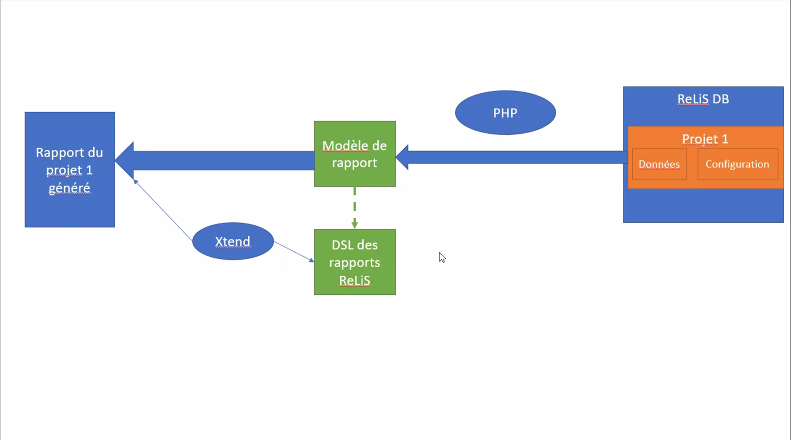
\includegraphics[width=0.65\textwidth]{resources/images/approach.PNG}
        \noskipcaption{Approche de résolution.}
\end{figure}

\newpage

\section{Mise en oeuvre}

\vspace*{3mm}

\subsection{Définition de la DSL}
La DSL est implémentée textuellement avec Xtext. On fait abstraction ici d'où proviennent les données et on se concentre sur les deux phases les plus importantes pour nous dans le rapport, à savoir le screening dans son ensemble et la classification, ainsi que les participants et leurs rôles dans le projet. Le méta-modèle généré à partir de la DSL ci-dessous va nous aider à mieux comprendre.

\begin{figure}[H]
        \centering
        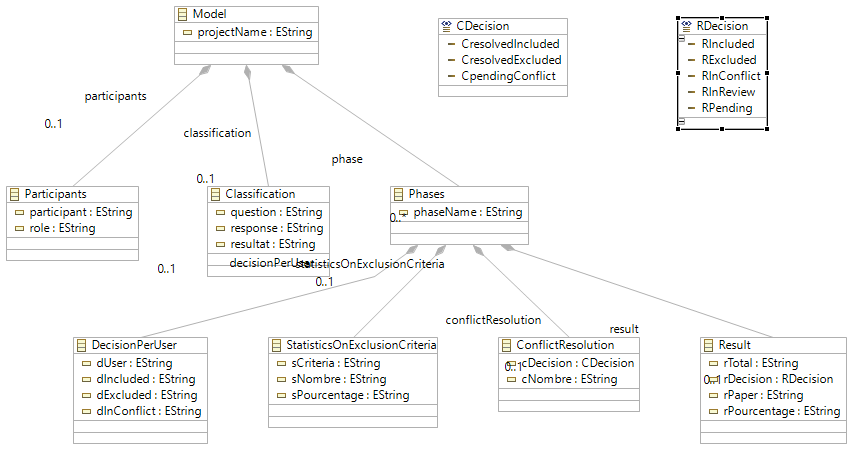
\includegraphics[width=0.65\textwidth]{resources/images/DSL.PNG}
        \noskipcaption{méta-modèle de la DSL}
\end{figure}

Notre modèle, qui représente un projet, se compose de 3 éléments principaux:
\begin{description}
    \item[Participants :] cette classe assure de renseigner chaque participant et sa fonction dans le projet.
    \item[Classification :] cette classe, quant à elle, va regrouper chaque question avec sa(ses) réponse(s) attendue(s), et le résultat, qui lui, représente le nombre d'article en accord avec l'affirmation de la réponse.
    \item[Phases :] étant donné que c'est un rapport d'un projet ReliS, les phases, qui sont celles du screening, fonctionnent avec la même logique que les phases de ReliS. Chaque phase contient la décision d'inclusion et d'exclusion de chaque participant du projet, les critères automatiques d'exclusion, la résolution des conflits et les résultats. 
\end{description}

\vspace*{3mm}

\subsection{Transformation Xtend vers le rapport}
Xtext a son propre générateur de code, Xtend, qui peut intervenir sur la DSL directement et utiliser les éléments dont on a besoin pour générer le code dont on a besoin. C'est avec cette technologie qu'on a généré le rapport. On verra par la suite le format du rapport avec plus de détails. Notons toutefois que l'artefact textuel généré pour le rapport est en \LaTeX{} et peut être compilé et être généré en pdf notamment.
\newpage
\subsection{Récupération des données depuis la base de données}
Pour les besoins du projet et pour protéger les données des utilisateurs, on a pas établi une connexion avec l'application en production. On a donc créé une base de données locale et on a simulé une connexion à ReliS. \\
Notre base de données se constitue comme suit:
\begin{figure}[H]
        \centering
        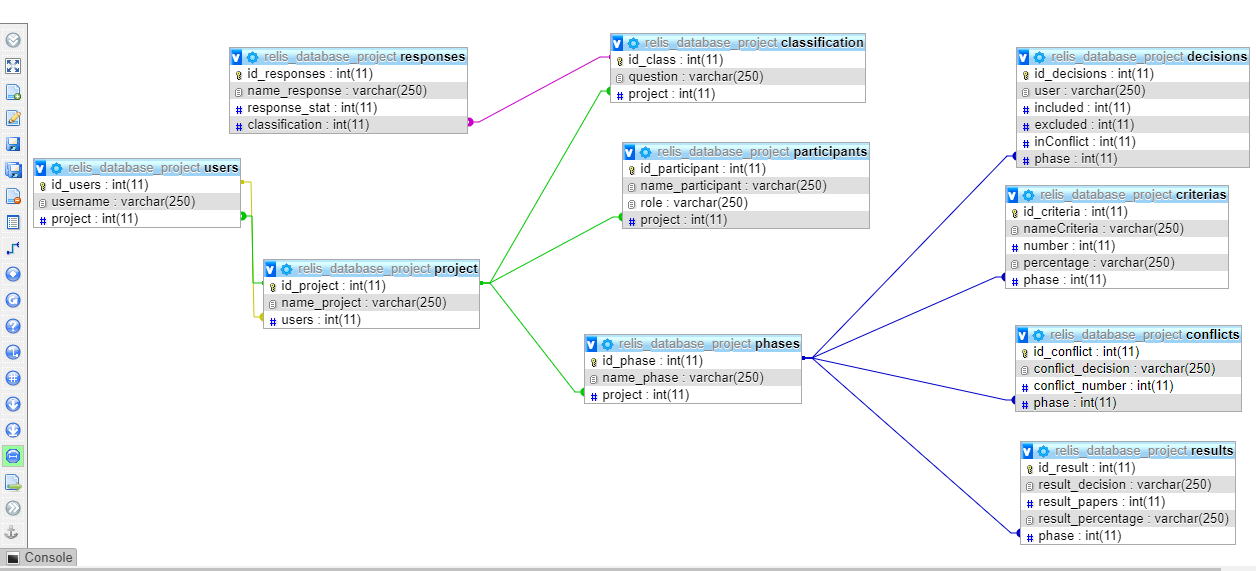
\includegraphics[width=0.65\textwidth]{resources/images/DB.PNG}
        \noskipcaption{base de données du projet}
\end{figure}

\vspace*{2mm}

La base de données est dans la même logique que la DSL. Un utilisateur(un compte relis) peut être associé à un ou plusieurs projets et un projet peut être associé à un ou plusieurs utilisateurs.
Suivant la logique de notre DSL, un projet est composé de 3 éléments principaux à savoir \textbf{les participants, les phases et la classification.}

\begin{description}
    \item[participants :] les participants leurs rôles chacun.
    \item[classification :] la classification(les questions de la classification) et les réponses.
    \item[phases :] les phases du screening et ses quatre composants principaux à savoir \textit{les décisions des participants, les critères, les conflits et les résultats}. 
\end{description}

L'implémentation de cette partie est faite en php avec une base de données MySQL.

\newpage

\section{Évaluation de notre solution}

Étant donné que notre travail est expérimental et qu'on simule une connexion à ReliS, on a copié un certain nombre de données de quelques projets pour l'expérimentation mais pas la totalité bien entendu vu que l'import des données n'est pas faisable et que l'accès aux données de l'application en production non plus, même via une API, étant donné qu'elle n'a pas été faite. Idéalement, ce serait toutes les données de ReliS et la démarche est la suivante:

\begin{enumerate}
    \item on va dans le site : \href{https://relis-project.bensoilih.com}{https://relis-project.bensoilih.com}
    \item on écrit son nom d'utilisateur, le même que celui de son compte ReliS suite à quoi les projets effectués ou ceux où on a participé s'affichent.
    \item on récupère le code généré, qui est l'instance de notre DSL.
    \item on crée un fichier instance de notre DSL dans lequel on colle le code récupéré, suite à quoi le code \LaTeX{} du rapport du projet sera généré.
    \item on peut compiler ce code en sortir un pdf.
\end{enumerate}

\newpage
Ci-dessous les personnes ayant des projets dans notre base de données pour la simulation et donc un projet ReliS dans notre solution. Ces données sont de réelles données des vrais projets de même nom sur ReliS.
Cette liste est fourni  à des fins de tests pour essayer notre solution.

\begin{figure}[H]
        \centering
        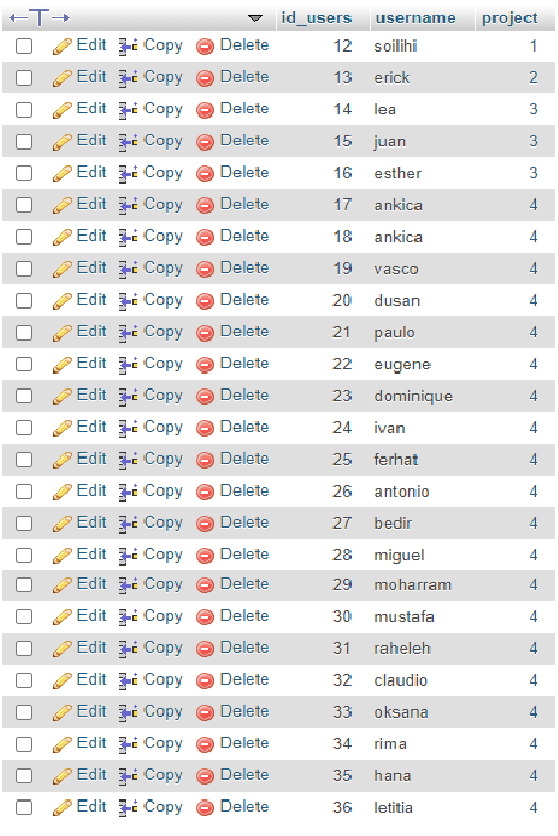
\includegraphics[width=0.65\textwidth]{resources/images/users.PNG}
        \noskipcaption{liste des personnes ayant un projet}
\end{figure}

\newpage

\subsection{Exemple avec notre projet}

Comme indiqué dans la première étape, on se rend dans le site : \href{https://relis-project.bensoilih.com}{https://relis-project.bensoilih.com} 
\vspace*{2mm}
Dans ce site, on écrit notre nom d'utilisateur, pour notre cas \textbf{soilihi} et on voit les projets dans lesquels la personne
est impliqué comme le montre la figure qui suit:

\begin{figure}[H]
        \centering
        
\includegraphics[width=0.65\textwidth]{resources/images/exemple1.PNG}
        \noskipcaption{listes des projets de soilihi}
\end{figure}

\vspace*{4mm}

Au clic de ce projet, un code est automatiquement généré et c'est le code d'une instance de notre DSL comme le montre la figure qui suit:

\begin{figure}[H]
        \centering
        
\includegraphics[width=0.65\textwidth]{resources/images/exemple2.PNG}
        \noskipcaption{code de l'instance de notre DSL}
\end{figure}

\newpage

Ensuite, après avoir récupéré ce code, on va dans Eclipse créer un fichier modèle de notre DSL avec l'extension \textbf{.slr} dans lequel on va coller le code récupéré précédemment comme l'illustre la suivante figure:

\begin{figure}[H]
        \centering
        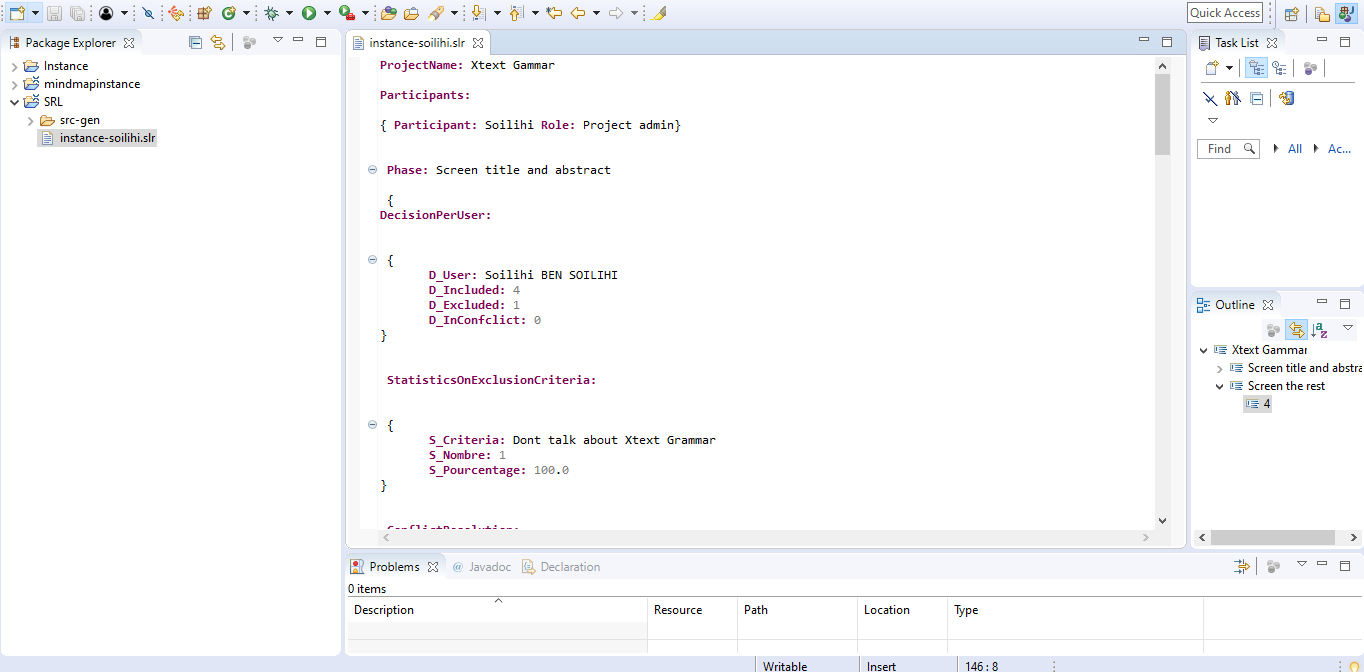
\includegraphics[width=0.65\textwidth]{resources/images/exemple3.PNG}
        \noskipcaption{code de l'instance de notre DSL}
\end{figure}

A la sauvegarde, un fichier avec le code latex du rapport se génère comme le montre la figure suivante:

\begin{figure}[H]
        \centering
        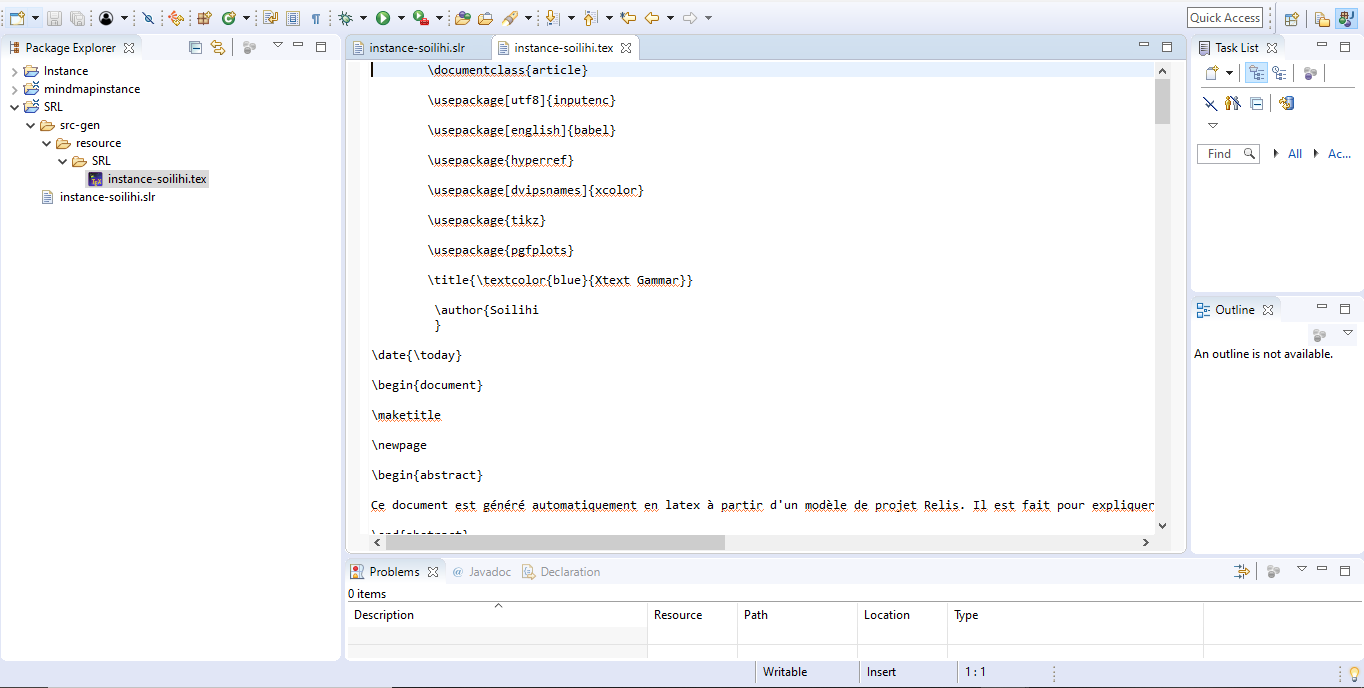
\includegraphics[width=0.65\textwidth]{resources/images/exemple4.PNG}
        \noskipcaption{code latex du rapport du projet}
\end{figure}

Ce code peut être compilé et sortir le rapport recherché comme on peut voir ci-dessous:

\begin{figure}[H]
        \centering
        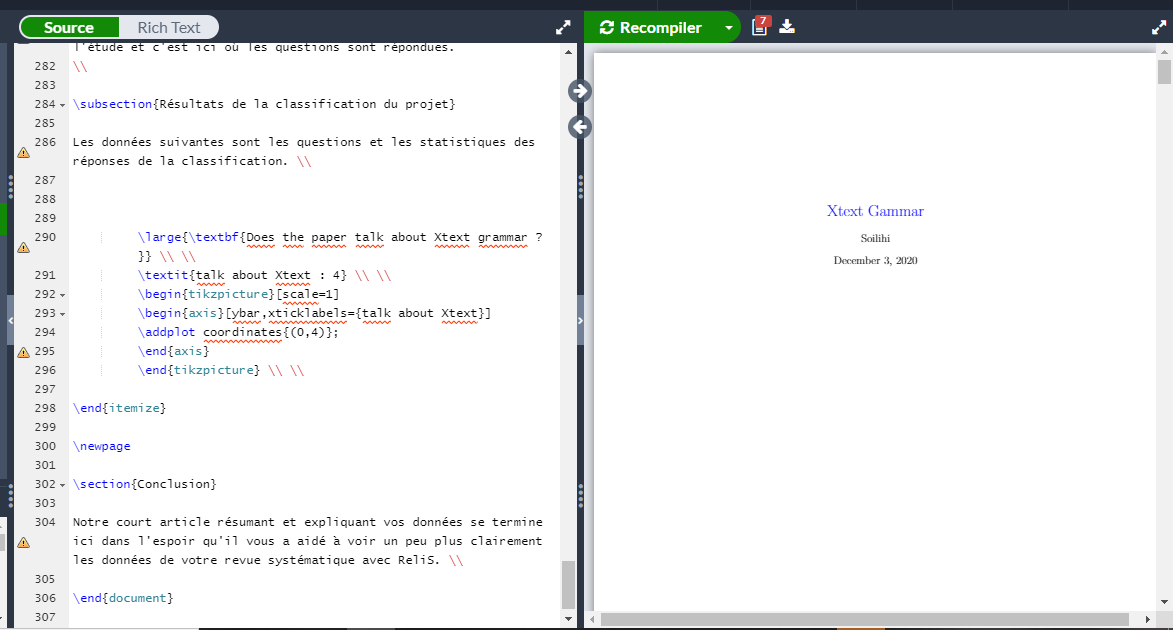
\includegraphics[width=0.65\textwidth]{resources/images/exemple5.PNG}
        \noskipcaption{rapport du projet Xtext Gammar}
\end{figure}
\newpage
\section{Constitution du rapport}

Le rapport se construit comme le montre l'image qui suit:

\begin{figure}[H]
        \centering
        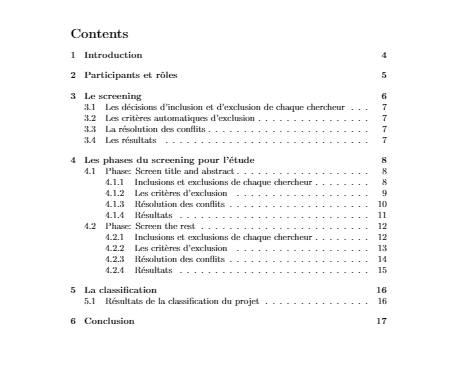
\includegraphics[width=0.65\textwidth]{resources/images/rapport.PNG}
        \noskipcaption{constituants du rapport}
\end{figure}
\vspace*{4mm}
\begin{itemize}
    \item Il est d'abord constitué d'une introduction, suivi des participants et leurs rôles
    \item puis des explications du screening,
    \item  puis les détails de chacun des phases du screening
    \item Vient ensuite la classification avant la conclusion.
\end{itemize}
Des explications sont présentes et des schémas pour aider à la compréhension.
\newpage
\section{Discussion sur notre travail}

Il y'a deux problèmes principaux sur le projet :
\begin{itemize}
    \item Le premier est que le projet est expérimental. Bien que les données soient des données réelles de ReliS, on a toutefois pas accès aux données de l'application en production ce qui fait qu'on a ça comme première limitation. Si une API pour l'accès aux données fut accessible, cela rendrait le projet encore plus efficace et surtout beaucoup plus utile.
    \item le second est que le processus n'est pas automatisé. Bien qu'il ait plusieurs générations et aucun code à écrire pour utiliser notre solution, il y'a toutefois beaucoup de choses à faire à la main comme copier les codes et les coller aux endroits appropriés.
    \end{itemize}
\vspace*{4mm}
\newpage
\section{Travaux connexes}

Nos recherches sur des travaux faisant ou ayant fait la même chose pour ReliS n'ont pas été fructueuses. Notre travail pourrait être le premier point d'appui pour des travaux futurs allant dans ce sens.
\newpage
\section{Conclusion}
\vspace*{0.4cm}
\hspace*{0.8cm}
Les revues systématiques sont d'une importance capitale dans le monde de la recherche et les réaliser peut-être une tâche ardue. ReliS aide à faire le processus de manière automatisée avec une approche d'ingénierie dirigée par les modèles. Il génère des résultats de ces revues séparés en phases pour le screening et la classification.
Rendre les données de tels travaux assemblées, structurées et avec des explications ne peut qu'être bénéfique pour la recherche et rajouter de la valeur au merveilleux outil qu'est ReliS. 
Notre travail s'est concentré sur cet aspect là et a essayé d'y apporter une première solution. Toutefois, quelques problèmes d'accès aux vraies données nous donne une limitation et automatiser le processus rendrait le travail plus efficace.

\newpage

\printbibliography

\end{document}
